% documentclass: article used for scientific journals, short reports, program documentation, etc
% options: fontsize 11, generate document for double sided printing, a4-paper
\documentclass[9pt, twoside, a4paper, fleqn, twocolumn]{extarticle}

\usepackage{extsizes}

% package for changing page layout
\usepackage{geometry}
\geometry{a4paper, lmargin=27mm, rmargin=27mm, tmargin=30mm, bmargin=45mm}
% set indentation
\setlength{\parindent}{1em}
% set factor for line spacing
% \linespread{1.4}\selectfont
% set (dynamic) additional line spacing
% \setlength{\parskip}{1ex plus 0.5ex minus 0.3ex}

% rigorous formatting (not too much hyphens)
% \fussy
% \sloppy

% package for changing page layout (used to indent whole paragraphs with adjustwidth)
\usepackage{changepage}

% input encoding for special characters (e.g. ä,ü,ö,ß), only for non english text
% options: utf8 as encoding standard, latin1
\usepackage[utf8]{inputenc}
% package for font encoding
\usepackage[T1]{fontenc}
% package for changing used language (especially for more than one language)
% options: ngerman (new spelling) or default: english
\usepackage[german]{babel}
% package for times font
% \usepackage{times}
% package for latin modern fonts
% \usepackage{lmodern}

% package for math symbols, functions and environments from ams(american mathematical society)
\usepackage{amsmath}
\usepackage{mathtools}
% package for extended symbols from ams
\usepackage{amssymb}
% package for math black board symbols (e.g. R,Q,Z,...)
\usepackage{bbm}
% package used for calligraphic math symbols
\usepackage{mathrsfs}
% package for extended symbols from stmaryrd(st mary road)
\usepackage{stmaryrd}
% package for more math blackboard symbols
\usepackage{dsfont}

% package defines commands \degree,\celsius for units 
\usepackage{gensymb}

% pack­age im­ple­ments scal­ing of the math ex­ten­sion font cmex; used for scaling math signs
\usepackage{exscale}

% package for including extern graphics plus scaling and rotating
\usepackage{graphicx}

% package for positioning figures
\usepackage{float}
% package includes command \FloatBarrier for float-figures; option: section adds barrier for every section, above allows floats to appear above the barrier on the same page
% \usepackage[section,above]{placeins}
\usepackage{placeins}

% package for changing color of font and paper
% options: using names of default colors (e.g red, black)
% \usepackage[usenames]{color}
\usepackage[dvipsnames]{xcolor}
\definecolor{shadecolor}{gray}{0.9}

% package for customising captions
\usepackage[footnotesize, hang]{caption}
% package for subfigures and subcaptions
\usepackage[font=footnotesize,format=hang]{subcaption}
%\captionsetup[sub]{format=hang}

% package for quotation marks in different languages (use \enquote)
\usepackage[autostyle,german=guillemets]{csquotes}

% package for customising enumerations (e.g. axioms)
\usepackage{enumitem}

% calc package reimplements \setcounter, \addtocounter, \setlength and \addtolength: commands now accept an infix notation expression
\usepackage{calc}

% package for creating framed, shaded, or differently highlighted regions that can break across pages; environments: framed, oframed, shaded, shaded*, snugshade, snugshade*, leftbar, titled-frame
\usepackage{framed}

% package for creating custom "list of"
% options: titles: do not intefere with standard headings for "list of"
\usepackage[titles]{tocloft}

% change enumeration style of equations
% \renewcommand\theequation{\thesection.\arabic{equation}}


% provides \ifthenelse command
\usepackage{ifthen}
% extra commands for if-conditions (e.g. \isempty)
\usepackage{xifthen}

% init list of math for definitions and theorems
\newcommand{\listofmathcall}{Verzeichnis der Definitionen und Sätze}
\newlistof{math}{mathlist}{\listofmathcall}
% add parentheses around argument
\newcommand{\parent}[1]{ \ifx&#1&\else (#1) \fi }
\definecolor{mathdefback}{rgb}{0.95,0.95,0.98}
% unnumerated mathematical definition environment definiton
\newenvironment{mathdef*}[2]{
	\medskip
	\begin{tcolorbox}[colback=mathdefback, boxrule=0.5pt, colframe=black, boxsep=0pt, enhanced jigsaw, breakable, arc=3pt]
	\noindent
	{ \fontfamily{ppl}\selectfont \textbf{\textsc{#1:}} } ~ #2 
	\par \hfill\\ 
	\fontfamily{lmr}\selectfont \itshape
}{
	\end{tcolorbox}
	\medskip
}
% definitions for numerated mathematical definition environment
\newcounter{mathdefc}[section]
\newcommand*{\mathdefnum}{\thesection.\arabic{mathdefc}}
\renewcommand{\themathdefc}{\mathdefnum}
\newenvironment{mathdef}[2]{
	\refstepcounter{mathdefc}
	\addcontentsline{mathlist}{figure}{\protect{\numberline{\mathdefnum}#1 ~ #2}}
	\begin{mathdef*}{#1 \mathdefnum}{#2}
}{
	\end{mathdef*}
}
% standard mathdef calls
\newcommand{\definitioncall}{Definition}
\newenvironment{definition*}[1][]{ \begin{mathdef*}{\definitioncall}{\parent{#1}} }{ \end{mathdef*} }
\newenvironment{definition}[1][]{ \begin{mathdef}{\definitioncall}{\parent{#1}} }{ \end{mathdef} }

\definecolor{maththeoremframe}{rgb}{0.7,0.7,0.73}

% unnumerated theorem environment definition
\newenvironment{maththeorem*}[2]{
	\medskip
	\begin{tcolorbox}[boxrule=0pt, leftrule=2.5pt, arc=2pt, colback=white, colframe=maththeoremframe, enhanced jigsaw, breakable, vfill before first, top=0mm, bottom=0mm, left=2mm, right=0mm, boxsep=1mm]
	\noindent
	{ \fontfamily{ppl}\selectfont \textbf{\textsc{#1:}} } ~ #2
	\par \hfill\\ 
	\fontfamily{lmr} \fontshape{it} \selectfont
}{ 
	\end{tcolorbox}
	\medskip
}
% definitions for numerated theorem environment
\newcounter{maththeoremc}[section]
\newcommand*\maththeoremnum{\thesection.\arabic{maththeoremc}}
\renewcommand{\themaththeoremc}{\maththeoremnum}
\newenvironment{maththeorem}[2]{
	\refstepcounter{maththeoremc}
	\addcontentsline{mathlist}{figure}{\protect{\qquad\numberline{\maththeoremnum}#1 ~ #2}}
	\begin{maththeorem*}{#1 \maththeoremnum}{#2}
}{
	\end{maththeorem*}
}
% standard maththeorem calls
\newcommand{\theoremcall}{Theorem}
\newenvironment{theorem*}[1][]{ \begin{maththeorem*}{\theoremcall}{\parent{#1}} }{ \end{maththeorem*} }
\newenvironment{theorem}[1][]{ \begin{maththeorem}{\theoremcall}{\parent{#1}} }{ \end{maththeorem} }
\newcommand{\lemmacall}{Lemma}
\newenvironment{lemma*}[1][]{ \begin{maththeorem*}{\lemmacall}{\parent{#1}} }{ \end{maththeorem*} }
\newenvironment{lemma}[1][]{ \begin{maththeorem}{\lemmacall}{\parent{#1}} }{ \end{maththeorem} }
\newcommand{\propositioncall}{Proposition}
\newenvironment{proposition*}[1][]{ \begin{maththeorem*}{\propositioncall}{\parent{#1}} }{ \end{maththeorem*} }
\newenvironment{proposition}[1][]{ \begin{maththeorem}{\propositioncall}{\parent{#1}} }{ \end{maththeorem} }
\newcommand{\corollarycall}{Korollar}
\newenvironment{corollary*}[1][]{ \begin{maththeorem*}{\corollarycall}{\parent{#1}} }{ \end{maththeorem*} }
\newenvironment{corollary}[1][]{ \begin{maththeorem}{\corollarycall}{\parent{#1}} }{ \end{maththeorem} }
% q.e.d. definition
\newcommand{\qed}{ \par \hfill \fontfamily{lmr} \fontshape{it} \selectfont \mbox{q.e.d.} \\}
\newcommand{\qedbox}{ \hfill $\Box$ }
% proof environment definition for theorems
\newenvironment{mathproof}[2]{
	% \par\hfill\\
	\medskip
	% \noindent
	% \par
	% { \fontfamily{ppl}\selectfont \small \textsc{#1:} } ~ \parent{#2} \smallskip\\
	% \begin{adjustwidth}{1em}{}
	\begin{tcolorbox}[title= { \fontfamily{ppl}\selectfont \small \textsc{#1:} } ~ \parent{#2}, boxrule=0pt, colback=white, colframe=white, coltitle=black, breakable, boxsep=0mm, top=2mm, bottom=0mm, right=0mm, left=0mm, before upper={\parindent1em}]%
	\normalfont
	\small
}{ 
	\end{tcolorbox}
	% \end{adjustwidth} 
	% \qedbox
	\medskip
}
% standard mathproof calls
\newcommand{\proofcall}{Beweis}
\newenvironment{proof}[1][]{ \begin{mathproof}{\textbf{\proofcall}}{#1} }{ \qedbox \end{mathproof} }
\newcommand{\proofideacall}{Beweisidee}
\newenvironment{proofidea}[1][]{ \begin{mathproof}{\proofideacall}{#1} }{ \end{mathproof} }

% math environment for examples (not numerated)
\newcommand{\examplecall}{Beispiel}
% \newcommand{\examplebox}{\hfill $\blacksquare$}
\newcommand{\examplebox}{\hfill $\rule{5pt}{5pt}$}
% \newenvironment{example}[1][]{ \begin{mathproof}{\examplecall}{#1} }{ \end{mathproof} }
\newenvironment{example}[1][]{
	\medskip
	\normalfont
	\small
	\textsc{\examplecall}: ~ \parent{#1} \\
}{
	% \par
	\examplebox
	\par
	\medskip
}
% fast font types
\newcommand{\m}[1]{\mathrm{#1}}
\newcommand{\s}[1]{\mathcal{#1}}


% logical equivalent define
\newcommand{\logeq}{\mathrel{\vcentcolon\Longleftrightarrow}}


% define
\newcommand{\define}{\coloneqq}
% define sign from the right
\newcommand{\definedby}{\eqqcolon}
% function
\newcommand{\func}[3]{#1\colon#2\to#3}


% brackets
% curly brackets
\newcommand{\curlb}[1]{\left\{ #1 \right\}}
% box brackets
\newcommand{\boxb}[1]{\left[ #1 \right]}
% parentheses/curved brackets
\newcommand{\curvb}[1]{\left( #1 \right)}
% angle brackets
\newcommand{\angleb}[1]{\left\langle #1 \right\rangle}
% floor brackets
\newcommand{\floorb}[1]{\left\lfloor #1 \right\rfloor}
% ceil brackets
\newcommand{\ceilb}[1]{\left\lceil #1 \right\rceil}


% symbols for sets
% create sets
% \newcommand{\set}[2][]{ \curlb{#2 \ifx&#1&\else \enspace\middle\vert\enspace #1 \fi} }
\newcommand{\set}[2][]{ \curlb{#2 \ifthenelse{\isempty{#1}}{}{\enspace\middle\vert\enspace #1}} }
% standard sets
\newcommand{\SR}{\mathds{R}} % real numbers
\newcommand{\SC}{\mathds{C}} % complex numbers
\newcommand{\SN}{\mathds{N}} % natural numbers
\newcommand{\SZ}{\mathds{Z}} % integral numbers
\newcommand{\SQ}{\mathds{Q}} % rational numbers
\newcommand{\SFP}{\mathds{P}} % polynom functions
\newcommand{\SFC}{\mathrm{C}} % complex valued functions (continous or differentiable)
\newcommand{\SFL}{\mathcal{L}} % space of integrable functions
\newcommand{\SFLL}{\mathrm{L}} % space of integrable function classes
% set of linear maps
\newcommand{\LM}{L}
% hilbert space
\newcommand{\SH}{\mathcal{H}}
% set of matrices
\newcommand{\SM}{\mathrm{M}}
% set of invertible
\newcommand{\SGL}{\mathrm{Gl}}
% group of orthogonal matrices
\newcommand{\SO}{\mathrm{O}}
% special group of orthogonal matrices
\newcommand{\SSO}{\mathrm{SO}}
% group of unitary matrices
\newcommand{\SU}{\mathrm{U}}
% hauptraum/generalized eigenspace
\newcommand{\hau}{\mathrm{Hau}}


% elements
% identity
\DeclareMathOperator{\id}{id}
% identity matrix
\newcommand{\idmat}{\mathrm{I}}
% normal distribution
\newcommand{\FN}{\mathcal{N}}


% operators
% inverse
\newcommand{\inv}[1]{ {#1}^{-1} }
% magnitude/absolute value
\newcommand{\abs}[1]{\left\vert #1 \right\vert}
% norm
\newcommand{\norm}[1]{\left\| #1 \right\|}
% power of set
\DeclareMathOperator{\setpow}{\mathcal{P}}
% real part
\DeclareMathOperator{\real}{Re}
% imaginary part
\DeclareMathOperator{\imag}{Im}
% complex conjugate
\newcommand{\conj}[1]{ \overline{#1} }
% diagonal matrix
\DeclareMathOperator{\diag}{diag}
% trace of matrix
\DeclareMathOperator{\tr}{tr}
% kernel of function
% \DeclareMathOperator{\ker}{ker}
% image of function
\DeclareMathOperator{\im}{im}
% annihilator
\DeclareMathOperator{\ann}{ann}
% transponent matrix
\newcommand{\transp}[1]{ {#1}^\m{T} }
% spectrum of matrix
\DeclareMathOperator{\spec}{\sigma}
% rank of matrix
\DeclareMathOperator{\rank}{rank}
% signum of permutation or number
\DeclareMathOperator{\sign}{sign}
% expectation
\DeclareMathOperator{\expect}{\mathbb{E}}
% variance
\DeclareMathOperator{\var}{var}
% covariance
\DeclareMathOperator{\cov}{cov}
% fourier transform
\newcommand{\fourier}{\mathcal{F}}
% derivative
\DeclareMathOperator{\Deriv}{D}
\newcommand{\deriv}[1]{ {#1}^{\prime} }
\newcommand{\dderiv}[1]{ {#1}^{\prime\prime} }
\newcommand{\ddderiv}[1]{ {#1}^{\prime\prime\prime} }
\newcommand{\nderiv}[2][]{ \ifx&#1& \deriv{#2} \else {#2}^{(#1)} \fi }
\DeclareMathOperator{\pderiv}{\partial}
% infinitesimal difference
\newcommand{\diff}{\mathrm{d}}
% integral
\newcommand{\integral}[4]{\int_{#1}^{#2} #3\ \diff #4}
\newcommand{\Integral}[4]{\int\limits_{#1}^{#2} #3\ \diff #4}
\newcommand{\iintegral}[2]{\int #1\ \diff #2} % indefinite integral
% scalar product
\newcommand{\dotp}[1]{\angleb{#1}}
% cross product sign
\newcommand{\cross}{\times}
% sign for direct sum
\newcommand{\dsum}{\oplus}
% linear span
\newcommand{\lspan}[1]{\angleb{#1}}
% dual space
\newcommand{\dual}[1]{ {#1}^* }
\newcommand{\ddual}[1]{ {#1}^{**} }
% bra-vector
\newcommand{\ket}[1]{ \left| #1 \right\rangle }
% ket-vector
\newcommand{\bra}[1]{ \left\langle #1 \right| }
% bracket
\newcommand{\bracket}[2]{ \left\langle #1 \middle| #2 \right\rangle }
% expectation of operator
\newcommand{\opexpect}[1]{ \angleb{#1} }

% converges arrow
\newcommand{\conv}[1][]{\xrightarrow[]{#1}}


% append unit
\newcommand{\unit}[1]{\, \mathrm{#1}}

% show formal atom with element name
\newcommand{\atom}[3][]{\prescript{#3}{#1}{\m{#2}}}
% show formal atom with variabel as name
\newcommand{\atomv}[3][]{\prescript{#3}{#1}{#2}}

%
\DeclareMathOperator*{\minimize}{minimise}



% package for init listings(non-formatted  text) e.g. different source codes
\usepackage{listings}


% definitions for listing colors
\definecolor{codeDarkGray}{gray}{0.2}
\definecolor{codeGray}{gray}{0.4}
\definecolor{codeLightGray}{rgb}{0.94,0.94,0.91}
\definecolor{codeBorder}{rgb}{0.34,0.24,0.21}
% predefinitions for listings
\newcommand{\listingcall}{Listing}
\newlength{\listingframemargin}
\setlength{\listingframemargin}{1em}
\newlength{\listingmargin}
\setlength{\listingmargin}{0.08\textwidth}
% \newlength{\listingwidth}
% \setlength{\listingwidth}{ ( \textwidth - \listingmargin * \real{2} + \listingframemargin * \real{2} ) }
% definitions for list of listings
\newcommand{\listoflistingscall}{\listingcall -Verzeichnis}
\newlistof{listings}{listinglist}{\listoflistingscall}
% style definition for standard code listings
\lstdefinestyle{std}{
	belowcaptionskip=0.5\baselineskip,
	breaklines=true,
	frameround=tttt,
	% frame=false,
	xleftmargin=0em,
	xrightmargin=0em,
	showstringspaces=false,
	showtabs=false,
	% tab=\smash{\rule[-.2\baselineskip]{.4pt}{\baselineskip}\kern.5em},
	basicstyle= \fontfamily{pcr}\selectfont\footnotesize\bfseries,
	keywordstyle= \bfseries\color{MidnightBlue}, %\color{codeDarkGray},
	commentstyle= \itshape\color{codeGray},
	identifierstyle=\color{codeDarkGray},
	stringstyle=\color{BurntOrange}, %\color{codeDarkGray},
	numberstyle=\tiny\ttfamily,
	% numbers=left,
	numbersep = 1em,
	% stepnumber = 1,
	% captionpos=t,
	tabsize=4,
	% backgroundcolor=\color{codebLightGray},
	rulecolor=\color{codeBorder},
	framexleftmargin=\listingframemargin,
	framexrightmargin=\listingframemargin
}
% definition for unnumerated listing
\newcommand{\inputlistingn}[3][]{
	\begin{center}
		\begin{adjustwidth}{\listingmargin}{\listingmargin}
			\centerline{ {\fontfamily{lmr}\selectfont \footnotesize \listingcall:}\quad {\footnotesize #2} }
			\lstinputlisting[style=std, #1]{#3}
		\end{adjustwidth}
	\end{center}
}
% definition for numerated listing
\newcounter{listingc}[section]
\newcommand*\listingnum{\thesection.\arabic{listingc}}
\renewcommand{\thelistingc}{\listingnum}
\newcommand{\inputlisting}[3][]{
	\refstepcounter{listingc}
	\addcontentsline{listinglist}{figure}{\protect{\numberline{\listingnum:} #2 } }
	% \inputlistingn[#1]{#2}{#3}
	\begin{center}
		\begin{adjustwidth}{\listingmargin}{\listingmargin}
			\centerline{ {\fontfamily{lmr}\selectfont \footnotesize \listingcall~\listingnum:}\quad {\footnotesize #2} }
			\lstinputlisting[style=std, #1]{#3}
		\end{adjustwidth}
	\end{center}
}


% package for including csv-tables from file
% \usepackage{csvsimple}
% package for creating, loading and manipulating databases
\usepackage{datatool}

% package for converting eps-files to pdf-files and then include them
\usepackage{epstopdf}
% use another program (ps2pdf) for converting
% !!! important: set shell_escape=1 in /etc/texmf/texmf.cnf (Linux/Ubuntu 12.04) for allowing to use other programs
% !!!			or use the command line with -shell-escape
% \epstopdfsetup{outdir=./}
% \epstopdfDeclareGraphicsRule{.eps}{pdf}{.pdf}{
% ps2pdf -dEPSCrop #1 \OutputFile
% }


% package for reference to last page (output number of last page)
\usepackage{lastpage}
% package for using header and footer
% options: automate terms of right and left marks
% \usepackage[automark]{scrpage2}
% \setlength{\headheight}{4\baselineskip}
% set style for footer and header
% \pagestyle{scrheadings}
% \pagestyle{headings}
% clear pagestyle for redefining
% \clearscrheadfoot
% set header and footer: use <xx>head/foot[]{Text} (i...inner, o...outer, c...center, o...odd, e...even, l...left, r...right)

% use that for mark to last page: \pageref{LastPage}
% set header separation line
% \setheadsepline[\textwidth]{0.5pt}
% set foot separation line
% \setfootsepline[\textwidth]{0.5pt}



\usepackage{tcolorbox}
% \usepackage{tikz}
% \tcbuselibrary{listings}
\tcbuselibrary{many}
\tcbset{fonttitle=\footnotesize}

\usepackage{array}

\allowdisplaybreaks

% \usepackage{epic, eepic}
\usepackage{epic}

\usepackage{natbib}
\bibliographystyle{alpha}
\usepackage{url}

% \usepackage{indentfirst}

\usepackage{titlesec}
\titleformat*{\section}{\large\bfseries}
\titlespacing*{\section}{0pt}{1.5\baselineskip}{0pt}
\titlespacing*{\subsection}{0pt}{\baselineskip}{0pt}
\titleformat*{\subsection}{\bfseries}

\usepackage{titling}
\title{}
\author{}

\usepackage{fancyhdr}
\fancypagestyle{titlestyle}{
	\fancyhf{}
	\fancyfoot[C]{\footnotesize\bigskip\thepage}
	% \fancyfoot{}
	\renewcommand{\footrulewidth}{0.5pt}
	\renewcommand{\headrulewidth}{0pt}
}

\fancypagestyle{mainstyle}{
	\fancyhf{}
	\fancyfoot[C]{\footnotesize\bigskip\thepage}
	\fancyhead[RO]{\footnotesize \leftmark} %left
	% \fancyhead[CE]{\footnotesize Prediction of Soil Parameters through Near Infrared Spectroscopy} %right
	\fancyhead[LE]{\footnotesize \leftmark} %right
	\renewcommand{\footrulewidth}{0.5pt}
	\renewcommand{\headrulewidth}{0.5pt}
}

\pagestyle{mainstyle}


\newcommand{\articletitle}{
	\thispagestyle{titlestyle}
	\hrule
	\section*{\centering \thetitle} % (fold)
	\noindent
	\parbox[b][][c]{0.5\textwidth}{\raggedright{\theauthor}}\hfill\parbox[b][][c]{0.5\textwidth}{\raggedleft{\email}}\\
	\hrule
	\bigskip
}

\usepackage{multirow}

\usepackage{csvsimple}
% \titleformat{\section}{\fontfamily{put}\selectfont}{\thesection}{1em}{}
 % \titleformat{\subsection}
    % {\normalfont\bf}{\thesection}{1em}{}
\usepackage{graphicx}
\usepackage{times}
% \usepackage{scrextend}
% \changefontsizes[9pt]{9pt}

\usepackage{datatool}



\title{Statistische Verfahren: \\ Projekt 4 - Nahinfrarotspektroskopie I}
\author{Tobias Giesemann \\ Ferdinand Rewicki \\ Moritz Preu\ss\@}
% \date{}
\newcommand{\email}{tobias.giesemann@uni-jena.de \\ ferdinand.rewicki@uni-jena.de \\ moritz.preuss@uni-jena.de}

\begin{document}
	\newgeometry{top=40mm,left=45mm,right=45mm}
	\onecolumn
	\maketitle
	\thispagestyle{empty}
	\hrule
	\medskip
	\begin{abstract}
		\itshape
		In der vorliegenden Arbeit wird eine Methode zur Ableitung einer Kalibierfunktion zur Bestimmung des Stickstoffgehalts in Bodenproben vorgestellt.
Basierend auf den zugrunde liegenden physikalischen und chemischen Eigenschaften der Nahinfrarotspektroskopie wird ein lineares Modell formuliert. 
Hierfür wurden potenzielle Prediktoren entsprechend ihrer Variabilität für das Maximalmodell ausgewählt und dann mit Hilfe von Mallow's Cp ein Idealmodell ermittelt. 
Darüber hinaus wurde der Einfluss des Stichprobenumfangs auf den durch den minimalen Cp-Wert geschätzten Vorhersagefehler untersucht.
	\end{abstract}
	\medskip
	\hrule
	\tableofcontents
	\newpage
	\null
	\thispagestyle{empty}
	\newpage
	\restoregeometry
	\pagenumbering{arabic}

	\linespread{1.1}\selectfont
	\twocolumn[
		{\begin{@twocolumnfalse}
			\thispagestyle{titlestyle}
			{\huge\bfseries \begin{center}{Statistische Verfahren: \\ Projekt 4.1 - Nahinfrarotspektroskopie I}\end{center}}
			\bigskip
			\begin{minipage}[t][][l]{0.33\textwidth}
				\centering{Tobias Giesemann \\ tobias.giesemann@uni-jena.de}
			\end{minipage}
			\hfill
			\begin{minipage}[t][][l]{0.33\textwidth}
				\centering{Ferdinand Rewicki \\ferdinand.rewicki@uni-jena.de}
			\end{minipage}
			\hfill
			\begin{minipage}[t][][l]{0.33\textwidth}
				\centering{Moritz Preu\ss\@ \\ moritz.preuss@uni-jena.de}
			\end{minipage}
			\bigskip
			\bigskip
			\hrule
			\medskip
			\begin{abstract}
				\itshape
				In der vorliegenden Arbeit wird eine Methode zur Ableitung einer Kalibierfunktion zur Bestimmung des Stickstoffgehalts in Bodenproben vorgestellt.
Basierend auf den zugrunde liegenden physikalischen und chemischen Eigenschaften der Nahinfrarotspektroskopie wird ein lineares Modell formuliert. 
Hierfür wurden potenzielle Prediktoren entsprechend ihrer Variabilität für das Maximalmodell ausgewählt und dann mit Hilfe von Mallow's Cp ein Idealmodell ermittelt. 
Darüber hinaus wurde der Einfluss des Stichprobenumfangs auf den durch den minimalen Cp-Wert geschätzten Vorhersagefehler untersucht.
			\end{abstract}
			\medskip
			\hrule
			\bigskip
			\bigskip
			\bigskip
		\end{@twocolumnfalse}}
	]

	\linespread{1.15}\selectfont
	
	%\thispagestyle{mainstyle}

	\section{Einleitung}
\label{sec:Einleitung}

    Die Zusammensetzung des Boden ist ein wesentlicher Faktor für einen ertragreichen und nachhaltigen Anbau von Pflanzen in der Landwirtschaft.
    Wichtige Parameter hierfür sind die Anteile des im Boden gebundenen Stickstoffs (N) und organische Kohlenstoffs (SOC), durch deren Messung Erkenntnisse über die Fruchtbarkeit des Bodens und die Auswirkungen der Bodennutzung gewonnen werden können.\cite{Poeplau2013}
    Die Messung der genannten Parameter ist durch sogenannte Fraktionierung von Bodenprobe möglich.
    Etablierte Messverfahren sind jedoch kostenintensiv, nicht vollständig standardisiert, und weisen eine schlechte Reproduzierbarkeit in verschiedenen Laboren auf.\cite{Poeplau2013}
    Aus diesem Grund sind Messverfahren notwendig, welche eine zuverlässige und effiziente Ermittlung der Menge des organischen Kohlenstoffs und gebundenen Stickstoffs im Bodens zulassen.
    Ein seit den sechziger Jahren vielfach eingesetztes Messverfahren ist die sogenannten Nahinfrarotspektroskopie. \cite{Agelet2010}
    Dieses erlaubt die Schätzung der nur aufwendig bestimmbaren Einflussparametern auf den Anteil von N (bzw.SOC) in Bodenproben mit Hilfe der leicht messbaren Nahinfrarotspektren.
    Die Bestimmung und Validierung eines hierfür notwendigen Modells für den Stickstoffgehalt in der Bodenprobe sind Gegenstand dieser Arbeit.
    Darüber widmet sich diese Arbeit einer statistischen Simulationsaufgabe: Es soll untersucht werden, inwiefern sich der SPSE-Wert (siehe Kapitel \ref{sec:Methodik}), der über Mallow's Cp geschätzt wird, verändert, wenn die zugrundeliegende Stichprobengröße erhöht wird.

% section Einleitung
	\section{Hintergrund}
\label{sec:Hintergrund}

	\subsection{Gebundener Stickstoff}
	\label{ssec:Gebundener Stickstoff}

	In der Natur geschieht eine fortwährender Austausch von Stickstoff zwischen Lebewesen, Boden und Atmosphäre.
	Ein Großteil des vorhandenen Stickstoffs liegt in gebundener Form im Erdboden vor und ist ein unentbehrlicher Nährstoff für Pflanzen und Lebewesen.
	Er wird von Pflanzen beim Wachstum aus der Erde aufgenommen und beim Absterben wieder freigesetzt.
    Zur Steigerung der Ernte ist eine Anreicherung des Bodens mit Nitrat durch der Einsatz von Düngemitteln daher gängige Praxis in der Landwirtschaft.\cite{Umweltbundesamt2017}
    Dies kann dann zu Problemen führen, wenn es zu einer Übersättigung des Bodens mit Stickstoff kommt.
    Durch Ausschwemmen des in Form von Nitrat ($NO_3^-$) und Ammonium ($NH_4^+$) gebundenen Stickstoffs kann dieser ins Grundwasser gelangen und eine Gefahr für die Umwelt darstellen.
    Sowohl für den Erfolg der Landwirtschaft als auch für den Schutz der Umwelt ist daher eine zuverlässige und effiziente Ermittlung des Nitratgehalts im Bodens von entscheidender Bedeutung.
    Der Messung des Stickstoffs liegen folgende chemische Zusammenhänge zu Grunde:


    Die Stoffmengenkonzentration von Stickstoff $c_{(N)}$ lässt sich berechnen durch
    	\[
			c^\m{(N)} \define \frac{n^\m{(N)}}{V}
		\]
		wobei $V$ das Volumen der Lösung und $n_{(N)}$ die enthaltenen Stoffmenge von Stickstoff ist.

    Für eine gegebene Stoffmengenkonzentration $c_0$ und Stoffmenge $n_o$ einer Probe, definieren wir den Stoffmengenanteil $y_\m{(N)}$ von Stickstoff als,
        \[
			y^\m{(N)} \define \frac{c^\m{(N)}}{c_0} = \frac{n^\m{(N)}}{n_0}
		\]

	% subsection Gebundener Stickstoff

	\subsection{Nahinfrarotspektroskopie}
	\label{ssec:Nahinfrarotspek}

		Bei der Nahinfrarotspektroskopie kommen elektromagnetische Wellen im Bereich zwischen 120 THz und 400 THz bzw. 2.500 nm und 750 nm zum Einsatz.\cite{Agelet2010}
		Das Messverfahren nutzt die Tatsache, dass bei der Bestrahlung einer Probe Teile des Lichts reflektiert, hindurch gelassen oder absorbiert werden.
		Von besonderem Interesse ist hierbei die Reflexion des Lichts, welche sich in die zwei Komponenten \glqq Spiegelreflexion\grqq{} und \glqq diffuse Reflexion\grqq{} unterscheiden lässt.
		Aus den Teilen des Lichts, welche diffus reflektiert werden, können aufgrund der größeren Eindringtiefe Informationen über die Beschaffenheit der Probe gewonnen werden.\cite{Agelet2010}
		Für eine Wellenlänge $\lambda$ ist das relative Reflexionsvermögen $\delta(\lambda)$ definiert als:
		\[
			\func{\delta}{(0,\infty)}{(0,\infty)},\qquad \delta(\lambda) \define \frac{P_\m{r}(\lambda)}{P_s}
		\]

		wobei $P_\m{r}(\lambda)$ die Reflexion einer Probe und $P_0$ die Reflexion eines Materials mit einem Reflexionsanteil nahe $100\%$ ist.

		Weiterhin lässt sich unter Anwendung des Beer'schen Gesetzes ein approximativer Zusammenhang zwischen dem relativen Reflexionsvermögen und der Stoffmenge $c_\m{(N)}$ des Stickstoffs herstellen.
		In eine Probe mit $n$ verschiedenen Stoffen sei $c_i$ die Stoffmengenkonzentration des $i$ten in der Probe enthaltenen Stoffes.
		Dann sei $\varepsilon_i(\lambda)$ ein Koeffizient mit $i\in\SN,i\leq n$ sodass
		\[
			-\log \delta(\lambda) = -\log \frac{P_\m{r}(\lambda)}{P_s} = \sum_{i=1}^{n} \varepsilon_i(\lambda) c_i
		\]


	% subsection Nahinfrarotspek

% section Hintergrund

	\thispagestyle{mainstyle}
	% !TeX spellcheck = de_DE
\section{Methodik}
\label{sec:Methodik}

	\subsection{Datensatz}
	\label{ssec:Datensatz}

	    Der für die Modellwahl verwendete Datensatz beinhaltet die logarithmierten relativen Reflexionswerte $-\delta(\lambda)$ bei Wellenlängen zwischen 1400 nm und 2672 nm in einem Abstand von 4 nm sowie die Stoffmengeanteile $y^{(N)}$, $y^{(SOC)}$ und entsprechenden pH-Werte von insgesamt 533 Proben.
	    Informationen über die chemische Zusammensetzung der Probe in den Reflexionswerten im Nahinfrarotbereich sind stark überlagert. \cite{Agelet2010}
	    Aus diesem Grund ist eine sorgfältige Auswahl relevanter Wellenlängen von besonderer Bedeutung für die Erstellung eines zuverlässigen Modells.


	% subsection Datensatz

	\subsection{Statistisches Modell}
	\label{ssec:Statistisches Modell}

	    Sei $n\in\SN$ die Größe des Datensatzes und $k\in\SN$ mit $k< n$ die Anzahl der Wellenlängen im Datensatz.
	    Entsprechend Abschnitt \ref{ssec:Datensatz} definieren wir dann die Einflussgröße $x_{ij}$ als für die $i$te Probe und $j$te Wellenlänge als
	    \[
			x_{ij} \define -\lg \delta_i(\lambda_j)
		\]
		für jedes $i,j\in\SN,i\leq n,j\leq k$.

	    Der Stoffmengenanteil des Stickstoffs  $y^{(N)}$ stellt die Zielgröße unseres späteren Modells dar.
	    Wie definieren hierfür den Vektor der Stoffmengenanteile $y_i$ der $i$ten Probe als den $n$-dimensionalen Vektor
		\[
			 y^{(N)} \define \curvb{y^\m{(N)}_i}
		\]

        Nachdem wir sowohl die Einflussgrößen als auch die Zielgröße für das lineare Modell definiert haben, lassen sich diese nun in Zusammenhang bringen.
        Es ist valide anzunehmen, dass sich die Zielgröße durch einen Linearkombination der Einflussgrößen beschreiben lässt.
        Hierfür definieren wir zunächst $Y^\m{(N)}$ als einen zufälligen Vektor von $y^\m{(N)}$ mit
        \[
			 \expect Y^\m{(N)} \define \beta_0 + \sum_{j=1}^k{x_{ij}\beta_j}
		\]

		Zudem ist es notwendig eine Variable $\varepsilon^\m{(N)}$ einzuführen welchen den Zufall der Messungen beschreibt.
	    In Matrixschreibweise lässt sich dies durch die Designmatrix $\mathbb{X} \in \SR^{n \times (k+1)}$, dem Parametervektor $\beta \in \SR^{k+1}$ und dem stochastisch  verteilten Parameter $\varepsilon^\m{(N)}$ wie folgt darstellen.
		\[
			Y^\m{(N)} = \mathbb{X}\beta + \varepsilon^\m{(N)}
		\]
		Für den Zufallsparameter $\varepsilon^\m{(N)}$ muss zudem gelten
		\[
			\expect \varepsilon^\m{(N)} = 0, \qquad \cov \varepsilon^\m{(N)} = (\sigma^2)^\m{(N)} \idmat
		\]
		wobei $(\sigma^2)^\m{(N)} \in (0,\infty)$.
		Weiterhin soll angenommen werden, dass $\varepsilon^\m{(N)}$ normalverteilt ist mit
	    \[
			\varepsilon^\m{(N)} \sim \FN \curvb{0,(\sigma^2)^\m{(N)}\idmat}
		\]
	    sodass sich für das Gesamtmodell gilt
		\[
			Y^\m{(N)} \sim \FN \curvb{\mathbb{X}\beta^\m{(N)},(\sigma^2)^\m{(N)} \idmat}
		\]

	% subsection Statistisches Modell

	\subsection{Statistische Modellwahl im Falle von NIR-Spektroskopie}
	\label{ssec:Statistische Modellwahl}
    	Seien $Y\in \rm I\!R^{n}$ die Zielgröße eines statistischen Modellwahlverfahrens und $X \in \rm I\!R^{n \times d}$ die Matrix von $d$ Einflussparametern und $n$ Beobachtungen.
    	Zur Wahl einer geeigneten Menge von Einflussparametern $x_i$ auf die Zielgröße $y_i$  wird im klassischen linearen Modell die Modellwahl über eine hierarchische Aufstellung von linearen Modellen erriecht.
    	Beginnend mit dem minimalen Modelle $E(Y_i) = \beta_0$ werden dem Modell nach und nach neue potenzielle Einflussparameter $x_{ik}$ hinzugefügt.
    	Zu jedem dieser neuen $x_{ik}$ wird dann eine Teststatistik aufgestellt, die darauf hinweist, ob der gewählte Parameter wichtig ist ist oder nicht.
    	Dabei ist die Nullhypothese, dass $x_{ik}$ keinen Einfluss auf die Zielgröße hat: $ H_0 = \beta_k = 0$ und wird abgelehnt, falls $H_1 = \beta_k \neq 0$ zutrifft.
    	Dies wird über die T-Teststatistik erreicht,  wobei für den Fall, dass $H_0$ richtig ist, gilt: $\frac{\hat{\beta_k}}{\sqrt{\sigma^2(X^TX)^{-1}_{kk}}} \sim t_{n-(k+1)}$.
    	Mit diesem Modellwahlverfahren ergeben sich einige Schwierigkeiten, wobei die für unseren Fall besonders schwerwiegenden herausgehoben werden: In dieser Arbeit haben wir es mit einer großen Anzahl potenzieller Einflussvariablen auf dem Nah-Infrarotspekturm zu tun.
    	A priori kann schwer eine inhaltliche Deutung vorgenommen werden, die gewisse Wellenlängen bevorzugt. Daher ist eine hierarchische Modellwahll mit wenigen, wohlüberlegten Einflussvariablen nicht möglich.
    	Demnach muss in dieser Arbeit die Anzahl der möglichen Einflussgrößen stark erhöht werden und hier bekommen wir ein Problem mit der T-Teststatistik.
    	Es ließen sich sehr viele unterschiedliche Kombinationen von Einflussgrößen aufstellen und in eine hierarchische Form bringen.
    	Doch da wir bei der T-Teststatistik ein $\underline{zufälliges}$ Intervall konstruieren, gegen das unsere Hypothese getestet wird, ist die Wahrscheinlichkeit bei oft wiederholten Tests fälschlicherweise die Nullhypothese abzulehnen steigend mit Anzahl der Versuche.
    	An ein automatisiertes Modellwahlverfahren, das in dieser Arbeit von Vorteil ist, ist also mittels des T-Tests nicht zu erreichen. (siehe Skript 11/2018)
    	Stattdessen bietet sich eine Modellwahl basierend auf dem erwarteten Prognosefehler ("sum of prediction squared error", SPSE) an:
    	\[
    		SPSE \define \expect \sum_{i=1}^{n} (Y_{i+n} - x_{i}^\m{(M)}\hat{\beta_i}^\m{(M)})^2
    	\]
    
    	Hierbei sind die Werte in $Y_{i+n}$ neue, potenzielle Beobachtungen zum Einflussvektor $x_i$ und $x_{i}^{(M)}\hat{\beta_i}^{((M)}$ ist sind die Prognosewerte aus dem Modell $M$.
    	Der Prognosefehler lässt sich in 3 Terme zerlegen: Einen irreduzierbaren Prognosefehler, der unabhängig von dem momentan betrachteten Modell ist, einen Biasterm, der die Abweichung des aktuellen Modells $M$ vom Prognosemodell als Summe der quadrierten Prognose-Verzerrungen anzeigt und einen Varianzterm, der die Ungenauigkeiten widerspiegelt, die sich aus der Schätzung von $(|M|+1)$ unbekannten Parametern ergibt.
    	Der SPSE lässt sich über unterschiedliche Wege berechnen / abschätzen, mithilfe neuer Beobachtungen (1), (wiederholter) Zerlegung der Ursprungsdaten in Test- und Trainingsdaten (2) oder mittels Schätzung basierend auf der Residuenquadratsumme ("residual squared sum", RSS), hier im Vergleich zu o.g. SPSE:
    
    	\[
    	    \expect RSS^\m{(M)} \define \sum_{i=1}^{n} \expect (Y_{i} - \hat{Y_i}^\m{(M)})^2
    	\]
    	\[
    	    SPSE^\m{(M)} \define \sum_{i=1}^{n} \expect (Y_{i+n} - \hat{Y_i}^\m{(M)})^2
    	\]
    
    	Es kann gezeigt werden, dass RSS den Wert von SPSE systematisch unterschätzt, dass diese Unterschätzung jedoch behoben werden kann (siehe Skript 12/2018):
    
        \[
    	    SPSE^\m{(M)} \define \expect RSS^\m{(M)} + 2\tilde{\sigma}_{\underline{full}}^2(|M|+1)
        \]
    
        wobei $\tilde{\sigma}_{full}^2$ die Varianz des größten Modells ist.

	% subsection Statistische Modellwahl

	\subsection{Mallow's $C_{p}$}
	\label{ssec:mallows-C_p}



	\subsection{Validierung des Modells}
	\label{ssec:model-validation}
        Ein geeigneter Parameter zur Messung der globalen Anpassungsgüte einer Regression ist $R^2$, definiert als \textbf{Quelle}
        \[
            {R^2}^{(M)} \define \frac {\sum_{i=1}^n \curvb{\hat{y}^{(M)}_i - \overline{y}}^2}{\sum_{i=1}^n \curvb{y_i - \overline{y}}^2}
        \]
        Dieser beschreibt den Anteil der durch die Regression erklärten Quadratsumme an der totale Quadratsumme und nimmt dadurch Werte zwischen 0 und 1 an.
        Während ein $R^2$ von 1 für einen perfekten linearen Zusammenhang steht bedeutet ein Wert von 0, dass kein linearer Zusammenhang vorliegt.
        Für das gewählte Modell ergibt sich ein Wert von \textbf{....}.
        Dies weißt auf eine relativ gute Anpassung durch das gewählte Modell hin. \textbf{zu prüfen}
        Zudem ist es sinnvoll neben dem Parameter $R^2$ ein Korrelationsdiagramm zwischen der durch das Modell geschätzten Ausprägung $\hat{y}_i$ und dem wahren Wert $y_i$ zu betrachten.
        \textbf{Einfügen von Grafik: Korrelationsdiagramm}
    
    


	% subsection model-validation

	\subsection{Theoretische Grundlagen der Simulation}
	\label{ssec:Theoretische Grundlagen der Simulation}

        Wie in Abschnitt \ref{ssec:Statistische Modellwahl} beschrieben gibt der SPSE den erwarteten Prognosefehler an.
        Es ist offensichtlich, dass dieser Wert möglichst gering sein sollte, um ein verlässliche Vorhersagen zu neuen Daten zu generieren.
     
        Im Allgemeine kann der SPSE mit Hilfe neuer Beobachtungen geschätzt werden.\cite{Schumacher Skript}
        Da diese nicht zur Verfügung stehen werden stattdessen neuen Pseudobeobachtungen der Zielgröße mit Hilfe des gewählten Modells generiert.
        Der aus der Pseudobeobachtungen geschätzte Prognosefehler kann der mit dem wahren wahren Prognosefehler des Modellsverglichen werden.
        Bei gegebenem Modells $M$ wird der wahre Prognosefehler durch
        \[
            SPSE^\m{(M)} \define  n \sigma^2 + \curvb{\abs{M}+1} \sigma^2
        \]
        berechnet.
        
        Der neue Vektor der Pseudobeobachtungen ist gegeben durch,
        \[
            \widetilde{Y} \define \widetilde{y}_i + \varepsilon
        \]
        wobei für den stochastisch verteilen Parameter $\varepsilon$ gilt
        \[
            \varepsilon \sim \FN \curvb{0,\sigma^2\idmat_n} 
        \]
        und als Varianz die Varianz des Modells angenommen wird.
        \[
            \sigma^2 \define \curvb{\tilde{\sigma}^2}^{(M)}
        \]
        Aus den generierten Pseudodaten wird ein neues bestes Modell $\widetilde{M}$ auf basierend auf dem kleinsten Cp-Wert ausgewählt, für dass gilt.
        \[
            \widetilde{Y} \sim \FN \curvb{\mathbb{X}\widetilde{\beta}, \sigma^2 I_n}
        \]
        Hierfür wird die Varianz als unbekannt angenommen.
        Neben dem Vergleich des wahren und geschätzten Prognosefehlers bei gleicher Stichprobengröße soll zudem überprüft werden welcher Einfluss die Änderung der Stichprobengröße auf den Wert des geschätzten SPSE hat.
        Hierzu werden die verschiedenen Stichprobengrößen von $n = (100, 200, 300, 400, 500, 533)$ gewählt und zufällig aus dem Datensatz ausgewählt.
        Um die Verzerrung der Ergebnisse durch zufällige Ausreißer zu vermeiden werden die Simulationen mehrfach durchgeführt.
        
        
	% subsection Theoretische Grundlagen der Simulation
% section methodology

	\section{Implementierung}
\label{sec:implementation}
\subsection{Modellwahl}
\label{ssec:impl:modelwahl}
\begin{figure*}[ht]
    \centering
    \begin{tikzpicture}
        \begin{axis}[ 
            ylabel = $var(\delta(\lambda))$,
            xlabel = $\lambda$,
            xmin=1400, xmax=2700,
            ymin=0, %ymax=800,
            legend pos = north west,
            scaled ticks = false,
            width = \textwidth,
            height = 8cm,
            ymajorgrids,
            xmajorgrids,
            cycle list name=auto
        ]
            \addplot +[stack plots=y, no marks, thick]
            table[x=x,y=y,col sep=comma] {plots/data/slopeValues.csv};
            \addlegendentry{{\scriptsize Variablität}}
            
            \addplot +[ycomb, no marks, dashed] 
            table[x=x, y expr=0.0105 ,col sep=comma] {plots/data/selectedFeatures.csv};
            
            \begin{scope}[]
                \draw[] ({rel axis cs:1,0}|-{axis cs:0,0.001}) -- ({rel axis cs:0,0}|-{axis cs:0,0.001});
            \end{scope}
        \end{axis}
    \end{tikzpicture}
    \captionof{figure}{Variablität der Reflektionswerte. Die horizontale Linie markiert den Schwellwert von 0.001, die vertikalen Linien die im optimalen Modell enthaltenen Features. }
    \label{fig:selected_feat}
\end{figure*}

Wie in Abschnitt \ref{ssec:modellselektion} beschrieben, benötigen wir zur Auswahl der relevanten Prädiktoren die erste Ableitung der Reflektionswerte. Die Methode \textit{getSlope} berechnet diese als Differenz benachbarter Messwerte. Daraus ergibt sich in Methode \textit{criterionSlopeDist} die Variabilität je Wellenlänge als Differenz des größten und des kleinsten Wertes. Alle Wellenlängen mit einer Variablität größer einem vorgegebenen Schwellwert (hier: $0.001$) werden in Methode \textit{selectFeatures} für das Maximalmodell ausgewählt. Alle ausgewählen Variablen gehen linear in das Maximalmodell ein.\\
Mittels der im Paket \text{leaps} bereitgestellten Methode \text{regsubsets} wird aus dem 149 Prädiktoren umfassenden Maximalmodell das Modell als Bestes bestimmt, welches den kleinsten $C_p$ Wert aufweist. Die Variablen sowie die geschätzen Parameter des ausgewählen Modells sind in Tabelle \ref{table:model_parameters} dargestellt.\\

\subsection{Simulation}
\label{ssec:impl:simulation}
Das so ausgewählte, optimale Modell wird nun verwendet, um Pseudobeobachtungswerte zu simulieren. Die Simulation erfolgt in mehreren Runden und für verschiedene Stichprobengrößen von 150, 200, 250, 300, 350, 400, 450 und 500 zufällig ausgewählten sowie für die gesamten 533 Spektren des vorliegenden Datensatzes. In Methode \textit{simulateOnDatSubset} erfolgt zunächst die zufällige Auswahl der übergebenen Anzahl an Sprektren. Anschließend wird das unter Abschnitt \ref{ssec:impl:modelwahl} bestimmte, optimale Modell verwendet, um neue Stockstoffwerte zu erzeugen, wobei, wie in Abschnitt \ref{ssec:Theoretische Grundlagen der Simulation} beschrieben, eine Normalverteilung der Zufallsgröße angenommen wird. In jedem Simulationsdurchlauf wird der Ergebnisvektor als arithmetisches Mittel aus 1000 Durchgängen erzeugt. \\
Mit den so erzeugten Pseudobeobachtungen, sowie den originalen Reflektionswerten wird nun ein zweites mal die Methode \textit{regsubsets} aus dem \textit{leaps} Paket aufgerufen, um für den neuen Datensatz das beste Modell mittels Mallows' $C_p$-Kriterium zu bestimmen. Für jedes beste Modell wird die Modellgröße sowie der $C_p$-Wert erfasst.\\
Im Anschluss an die Somulation erfolgt die Berechnung des erwarteten Prognosefehler, welche in Methode \textit{calculateTrueSpse} nach Formel (\ref{eq:spse_true}) erfolgt. Die Schätzung des erwarteten Prognosefehlers aus den CP Werten der Simulation erfolgt in Methode \textit{calculateEstimatedSpse} nach der Formel
\[
\hat{\m{SPSE}}^{\m{(M)}} \define (C_p^{\m{(M)}} + (|M| + 1)) \Tilde{\sigma}^2_{full}
\]
		
% section implementation
	\section{Ergebnisse und Diskussion}
\label{sec:discuss}

\subsection{Modellwahl}
\label{ssec:discuss:modelselect}
Unter Anwendung der in Abschnitt \ref{ssec:modellselektion} bzw \ref{ssec:impl:modelwahl} vorgestellten Methode wurde aus einem 149 Prädiktoren umfassenden Maximalmodell das in Tabelle \ref{table:model_parameters} angegebene, 50 Prädiktoren große Modell anhand des kleinsten $C_p$-Wertes von $\m{\approx3.92}$ als optimales Modell ausgewählt.\\
\begin{figure*}[ht]
    \centering
    \begin{tikzpicture}
        \begin{axis}[ 
            ylabel = $N_{origin}$,
            xlabel = $N_{est}$,
            xmin=0, xmax=0.8,
            ymin=0, ymax=0.8,
            legend pos = north west,
            scaled ticks = false,
            width = .5\textwidth,
            ymajorgrids,
            xmajorgrids,
            %height = 8cm,
            cycle list name=black white
        ]
            \addplot +[only marks]
            table[x=origN, y=simN, col sep=comma] {plots/data/correlation_plot_data.csv};
            %\addlegendentry{{\scriptsize Variablität}}
            \begin{scope}[red]
                \draw[red] ({axis cs:0,0}) -- ({axis cs:1,1});
            \end{scope}   
            %\addplot +[ycomb, no marks, dashed] 
            %table[x=x, y expr=0.0105 ,col sep=comma] {plots/data/selectedFeatures.csv};
            
            
        \end{axis}
    \end{tikzpicture}
    \captionof{figure}{Korrelationsplot}
    \label{fig:correlation}
\end{figure*}
Der Wert des Bestimmtheitsmaßes $R^2 = 0.82$ zeigt, dass das gewählte Modell die Varianz in den Daten gut erklären kann. 
Dies spiegelt auch das in Abbildung \ref{fig:correlation} abgebildete Korrelationsdiagramm wieder.
Abweichungen sind lediglich im oberen Bereich ab $0.3$ zu beobachten, wo der Stoffmengenanteil des Stickstoffs durch das Modell unterschätzt wird.
Dies lässt sich vermutlich durch die geringe Datendichte in diesen Bereichen erklären.
Insgesamt kann man sagen, dass die bisherigen Untersuchungen auf ausreichend gute Prognosen durch das Modell hindeuten.

\begin{figure*}[ht]
    \centering
    \begin{tikzpicture}
        \begin{axis}[ 
            ylabel = N,
            xlabel = simN,
            xmin=0, xmax=600,
            ymin=0, ymax=1.5,
            legend pos = north west,
            scaled ticks = false,
            width = .5\textwidth,
            ymajorgrids,
            xmajorgrids,
            %height = 8cm,
            cycle list name=black white
        ]
            \addplot +[only marks]
            coordinates {
                (150,0.4964226)
                (200,0.4312206)
                (250,0.5213190)
                (300,0.6097658)
                (350,0.7058959)
                (400,0.7947748)
                (450,0.8807918)
                (500,0.9750933)
                (533,1.0280917)
            };
            \addlegendentry{{\scriptsize geschätzter SPSE}}
            
            \addplot +[only marks]
            coordinates {
                (533,0.9813258)
            };
            \addlegendentry{{\scriptsize wahrer SPSE}}
            
            %\addplot +[ycomb, no marks, dashed] 
            %table[x=x, y expr=0.0105 ,col sep=comma] {plots/data/selectedFeatures.csv};
        \end{axis}
    \end{tikzpicture}
    \captionof{figure}{SPSE}
    \label{fig:spse}
\end{figure*}

\subsection{Simulation}
\label{ssec:discuss:simulation}
Die vorliegende Arbeit sollte den Einfluss des Stichprobenumfangs auf die SPSE-Schätzung mithilfe Mallow's $C_p$ untersuchen. Die hier angegebenen Werte spiegeln den Mittelwert aus 10 Durchläufen wieder.

\begin{table}[!h]
    \centering
	\begin{tabular}{|l|l|}
		\cline{1-2}
		$n$   & $\hat{SPSE}$ \\ 		\cline{1-2}
		150 &  0.4964226   \\ \cline{1-2}
		200 &  0.4312206   \\ \cline{1-2}
		250 &  0.521319    \\ \cline{1-2}
		300 &  0.6097658  \\ \cline{1-2}
		350 &  0.7058959   \\ \cline{1-2}
		400 &  0.7947748 \\ \cline{1-2}
		450 &  0.8807918  \\ \cline{1-2}
		500 &  0.9750933   \\ \cline{1-2}
		533 &  1.028092   \\ \cline{1-2}

	\end{tabular}
	\caption{Über Mallow's $C_p$ geschätzte SPSE Werte mit zugehörigen $n$}
\end{table}

Wie in Abbildung \ref{fig:spse} zu erkennen ist steigt der geschätzte SPSE-Wert außer bei $n < 200$ monoton und nahezu linear mit zunehmender Stichprobengröße. Dies lässt auf einen starken linearen Einfluss von $n$ auf den SPSE schließen. In der Berechnung des SPSE ist $n$ sowohl als Faktor im unkontrollierten Prognosefehler als auch im Biasterm vorhanden, was den Einfluss auf das Ergebnis bereits vermuten ließ.
Der tatsächliche SPSE von 0,981 wird bei der Schätzung über Mallow's $C_p$ mit derselben Stichprobengröße (533) um knapp 5\% überschätzt und liegt bei 1,028. 
Daraus lässt sich schließen, dass der Biasterm durch die zufällige Simulation wohl leicht überschätzt wurde.
Wir können also schlussfolgern, dass SPSE Werte, die auf verschiedenen Stichprobengrößen beruhen, normiert werden müssen, um miteinander vergleichbar zu sein.


	%\section{Simulation}


	

% section simulation
	\section{Conclusion}
\label{sec:conclusion}

	Using Mallow's $C_\m{p}$ criterion, we calibrated three predictive models for the soil parameters $p^{(\m{SOC})}$, $p^{(\m{N})}$ and $\m{pH}$.
	To construct ...
	

% section conclusion
	
	\bibliography{ref}
	
	\appendix
	\onecolumn
	\pagenumbering{roman}
	\section{Prediction Parameters and Models}
\label{sec:parameters}

	\begin{table}[H]
		\center
		\caption{Estimated model parameters of $P^\m{(SOC)}$ on selected model}
		\setlength{\extrarowheight}{1.9pt}
		\begin{tabular}{rr|rr|rr|rr}
			\hline
			$\lambda_i \ [\m{nm}]$ & $\beta^\m{(SOC)}_i$ & $\lambda_i \ [\m{nm}]$ & $\beta^\m{(SOC)}_i$ & $\lambda_i \ [\m{nm}]$ & $\beta^\m{(SOC)}_i$ & $\lambda_i \ [\m{nm}]$ & $\beta^\m{(SOC)}_i$ \\
			\hline
			\hline
%			--- & -1.47103 & 1808 & 1991.63 & 2204 & -2319.71 & 2496 & 1956.13\\
1424 & -811.326 & 1828 & 1568.91 & 2216 & 1075.21 & 2508 & -5057.56\\

			\hline \\
		\end{tabular}
	\end{table}

	\begin{table}[H]
		\center
		\caption{Estimated model parameters of $\overline{\m{pH}}$ on selected model}
		\setlength{\extrarowheight}{1.9pt}
		\begin{tabular}{rr|rr|rr|rr}
			\hline
			$\lambda_i \ [\m{nm}]$ & $\beta^\m{(pH)}_i$ & $\lambda_i \ [\m{nm}]$ & $\beta^\m{(pH)}_i$ & $\lambda_i \ [\m{nm}]$ & $\beta^\m{(pH)}_i$ & $\lambda_i \ [\m{nm}]$ & $\beta^\m{(pH)}_i$ \\
			\hline
			\hline
%			--- & 5.57628 & 1864 & -508.298 & 2220 & 699.185 & 2460 & 545.634\\
1436 & 135.244 & 1896 & -623.655 & 2224 & -659.264 & 2464 & -519.611\\


			\hline \\
		\end{tabular}
	\end{table}

	\begin{table}[H]
		\center
		\caption{Estimated model parameters of $P^\m{(N)}$ on selected model}
		\setlength{\extrarowheight}{1.9pt}
		\begin{tabular}{rr|rr|rr|rr}
			\hline
			$\lambda_i \ [\m{nm}]$ & $\beta^\m{(N)}_i$ & $\lambda_i \ [\m{nm}]$ & $\beta^\m{(N)}_i$ & $\lambda_i \ [\m{nm}]$ & $\beta^\m{(N)}_i$ & $\lambda_i \ [\m{nm}]$ & $\beta^\m{(N)}_i$ \\
			\hline
			\hline
%			--- & -0.0287506 & 1820 & 169.949 & 2156 & 95.2657 & 2428 & 116.231\\
1400 & 48.2214 & 1824 & -272.304 & 2184 & -99.54 & 2436 & -60.6976\\

			\hline \\
		\end{tabular}
	\end{table}


	\begin{figure}[H]
		\begin{subfigure}[b]{\textwidth}
			\centering
			% GNUPLOT: LaTeX picture with Postscript
\begingroup
  \makeatletter
  \providecommand\color[2][]{%
    \GenericError{(gnuplot) \space\space\space\@spaces}{%
      Package color not loaded in conjunction with
      terminal option `colourtext'%
    }{See the gnuplot documentation for explanation.%
    }{Either use 'blacktext' in gnuplot or load the package
      color.sty in LaTeX.}%
    \renewcommand\color[2][]{}%
  }%
  \providecommand\includegraphics[2][]{%
    \GenericError{(gnuplot) \space\space\space\@spaces}{%
      Package graphicx or graphics not loaded%
    }{See the gnuplot documentation for explanation.%
    }{The gnuplot epslatex terminal needs graphicx.sty or graphics.sty.}%
    \renewcommand\includegraphics[2][]{}%
  }%
  \providecommand\rotatebox[2]{#2}%
  \@ifundefined{ifGPcolor}{%
    \newif\ifGPcolor
    \GPcolorfalse
  }{}%
  \@ifundefined{ifGPblacktext}{%
    \newif\ifGPblacktext
    \GPblacktexttrue
  }{}%
  % define a \g@addto@macro without @ in the name:
  \let\gplgaddtomacro\g@addto@macro
  % define empty templates for all commands taking text:
  \gdef\gplbacktext{}%
  \gdef\gplfronttext{}%
  \makeatother
  \ifGPblacktext
    % no textcolor at all
    \def\colorrgb#1{}%
    \def\colorgray#1{}%
  \else
    % gray or color?
    \ifGPcolor
      \def\colorrgb#1{\color[rgb]{#1}}%
      \def\colorgray#1{\color[gray]{#1}}%
      \expandafter\def\csname LTw\endcsname{\color{white}}%
      \expandafter\def\csname LTb\endcsname{\color{black}}%
      \expandafter\def\csname LTa\endcsname{\color{black}}%
      \expandafter\def\csname LT0\endcsname{\color[rgb]{1,0,0}}%
      \expandafter\def\csname LT1\endcsname{\color[rgb]{0,1,0}}%
      \expandafter\def\csname LT2\endcsname{\color[rgb]{0,0,1}}%
      \expandafter\def\csname LT3\endcsname{\color[rgb]{1,0,1}}%
      \expandafter\def\csname LT4\endcsname{\color[rgb]{0,1,1}}%
      \expandafter\def\csname LT5\endcsname{\color[rgb]{1,1,0}}%
      \expandafter\def\csname LT6\endcsname{\color[rgb]{0,0,0}}%
      \expandafter\def\csname LT7\endcsname{\color[rgb]{1,0.3,0}}%
      \expandafter\def\csname LT8\endcsname{\color[rgb]{0.5,0.5,0.5}}%
    \else
      % gray
      \def\colorrgb#1{\color{black}}%
      \def\colorgray#1{\color[gray]{#1}}%
      \expandafter\def\csname LTw\endcsname{\color{white}}%
      \expandafter\def\csname LTb\endcsname{\color{black}}%
      \expandafter\def\csname LTa\endcsname{\color{black}}%
      \expandafter\def\csname LT0\endcsname{\color{black}}%
      \expandafter\def\csname LT1\endcsname{\color{black}}%
      \expandafter\def\csname LT2\endcsname{\color{black}}%
      \expandafter\def\csname LT3\endcsname{\color{black}}%
      \expandafter\def\csname LT4\endcsname{\color{black}}%
      \expandafter\def\csname LT5\endcsname{\color{black}}%
      \expandafter\def\csname LT6\endcsname{\color{black}}%
      \expandafter\def\csname LT7\endcsname{\color{black}}%
      \expandafter\def\csname LT8\endcsname{\color{black}}%
    \fi
  \fi
  \setlength{\unitlength}{0.0500bp}%
  \begin{picture}(7936.00,3400.00)%
    \gplgaddtomacro\gplbacktext{%
      \csname LTb\endcsname%
      \put(1078,704){\makebox(0,0)[r]{\strut{} 0.3}}%
      \csname LTb\endcsname%
      \put(1078,1190){\makebox(0,0)[r]{\strut{} 0.35}}%
      \csname LTb\endcsname%
      \put(1078,1676){\makebox(0,0)[r]{\strut{} 0.4}}%
      \csname LTb\endcsname%
      \put(1078,2163){\makebox(0,0)[r]{\strut{} 0.45}}%
      \csname LTb\endcsname%
      \put(1078,2649){\makebox(0,0)[r]{\strut{} 0.5}}%
      \csname LTb\endcsname%
      \put(1078,3135){\makebox(0,0)[r]{\strut{} 0.55}}%
      \csname LTb\endcsname%
      \put(1353,484){\makebox(0,0){\strut{} 1400}}%
      \csname LTb\endcsname%
      \put(2304,484){\makebox(0,0){\strut{} 1600}}%
      \csname LTb\endcsname%
      \put(3256,484){\makebox(0,0){\strut{} 1800}}%
      \csname LTb\endcsname%
      \put(4208,484){\makebox(0,0){\strut{} 2000}}%
      \csname LTb\endcsname%
      \put(5160,484){\makebox(0,0){\strut{} 2200}}%
      \csname LTb\endcsname%
      \put(6111,484){\makebox(0,0){\strut{} 2400}}%
      \csname LTb\endcsname%
      \put(7063,484){\makebox(0,0){\strut{} 2600}}%
      \put(176,1919){\rotatebox{-270}{\makebox(0,0){\strut{}$-\lg \varrho(\lambda)$}}}%
      \put(4374,154){\makebox(0,0){\strut{}$\lambda \ [\m{nm}]$}}%
    }%
    \gplgaddtomacro\gplfronttext{%
      \csname LTb\endcsname%
      \put(6587,2892){\makebox(0,0)[r]{\strut{}$P^\m{(SOC)}$}}%
    }%
    \gplbacktext
    \put(0,0){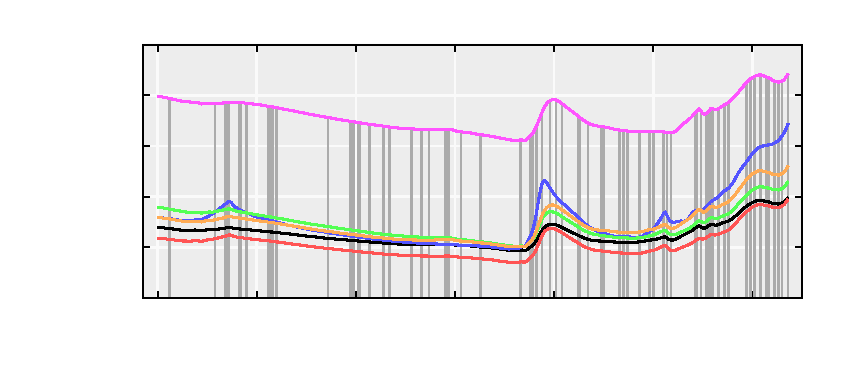
\includegraphics{gp/ms-sa-soc-spec-rnd}}%
    \gplfronttext
  \end{picture}%
\endgroup

			\caption{$p^{(\m{SOC})}$ with $\m{p}^{(\m{SOC})} = 72$}
			\label{sfig:calib-soc}
		\end{subfigure}

		\begin{subfigure}[b]{\textwidth}
			\centering
			% GNUPLOT: LaTeX picture with Postscript
\begingroup
  \makeatletter
  \providecommand\color[2][]{%
    \GenericError{(gnuplot) \space\space\space\@spaces}{%
      Package color not loaded in conjunction with
      terminal option `colourtext'%
    }{See the gnuplot documentation for explanation.%
    }{Either use 'blacktext' in gnuplot or load the package
      color.sty in LaTeX.}%
    \renewcommand\color[2][]{}%
  }%
  \providecommand\includegraphics[2][]{%
    \GenericError{(gnuplot) \space\space\space\@spaces}{%
      Package graphicx or graphics not loaded%
    }{See the gnuplot documentation for explanation.%
    }{The gnuplot epslatex terminal needs graphicx.sty or graphics.sty.}%
    \renewcommand\includegraphics[2][]{}%
  }%
  \providecommand\rotatebox[2]{#2}%
  \@ifundefined{ifGPcolor}{%
    \newif\ifGPcolor
    \GPcolorfalse
  }{}%
  \@ifundefined{ifGPblacktext}{%
    \newif\ifGPblacktext
    \GPblacktexttrue
  }{}%
  % define a \g@addto@macro without @ in the name:
  \let\gplgaddtomacro\g@addto@macro
  % define empty templates for all commands taking text:
  \gdef\gplbacktext{}%
  \gdef\gplfronttext{}%
  \makeatother
  \ifGPblacktext
    % no textcolor at all
    \def\colorrgb#1{}%
    \def\colorgray#1{}%
  \else
    % gray or color?
    \ifGPcolor
      \def\colorrgb#1{\color[rgb]{#1}}%
      \def\colorgray#1{\color[gray]{#1}}%
      \expandafter\def\csname LTw\endcsname{\color{white}}%
      \expandafter\def\csname LTb\endcsname{\color{black}}%
      \expandafter\def\csname LTa\endcsname{\color{black}}%
      \expandafter\def\csname LT0\endcsname{\color[rgb]{1,0,0}}%
      \expandafter\def\csname LT1\endcsname{\color[rgb]{0,1,0}}%
      \expandafter\def\csname LT2\endcsname{\color[rgb]{0,0,1}}%
      \expandafter\def\csname LT3\endcsname{\color[rgb]{1,0,1}}%
      \expandafter\def\csname LT4\endcsname{\color[rgb]{0,1,1}}%
      \expandafter\def\csname LT5\endcsname{\color[rgb]{1,1,0}}%
      \expandafter\def\csname LT6\endcsname{\color[rgb]{0,0,0}}%
      \expandafter\def\csname LT7\endcsname{\color[rgb]{1,0.3,0}}%
      \expandafter\def\csname LT8\endcsname{\color[rgb]{0.5,0.5,0.5}}%
    \else
      % gray
      \def\colorrgb#1{\color{black}}%
      \def\colorgray#1{\color[gray]{#1}}%
      \expandafter\def\csname LTw\endcsname{\color{white}}%
      \expandafter\def\csname LTb\endcsname{\color{black}}%
      \expandafter\def\csname LTa\endcsname{\color{black}}%
      \expandafter\def\csname LT0\endcsname{\color{black}}%
      \expandafter\def\csname LT1\endcsname{\color{black}}%
      \expandafter\def\csname LT2\endcsname{\color{black}}%
      \expandafter\def\csname LT3\endcsname{\color{black}}%
      \expandafter\def\csname LT4\endcsname{\color{black}}%
      \expandafter\def\csname LT5\endcsname{\color{black}}%
      \expandafter\def\csname LT6\endcsname{\color{black}}%
      \expandafter\def\csname LT7\endcsname{\color{black}}%
      \expandafter\def\csname LT8\endcsname{\color{black}}%
    \fi
  \fi
  \setlength{\unitlength}{0.0500bp}%
  \begin{picture}(7936.00,3400.00)%
    \gplgaddtomacro\gplbacktext{%
      \csname LTb\endcsname%
      \put(1078,704){\makebox(0,0)[r]{\strut{} 0.3}}%
      \csname LTb\endcsname%
      \put(1078,1190){\makebox(0,0)[r]{\strut{} 0.35}}%
      \csname LTb\endcsname%
      \put(1078,1676){\makebox(0,0)[r]{\strut{} 0.4}}%
      \csname LTb\endcsname%
      \put(1078,2163){\makebox(0,0)[r]{\strut{} 0.45}}%
      \csname LTb\endcsname%
      \put(1078,2649){\makebox(0,0)[r]{\strut{} 0.5}}%
      \csname LTb\endcsname%
      \put(1078,3135){\makebox(0,0)[r]{\strut{} 0.55}}%
      \csname LTb\endcsname%
      \put(1353,484){\makebox(0,0){\strut{} 1400}}%
      \csname LTb\endcsname%
      \put(2304,484){\makebox(0,0){\strut{} 1600}}%
      \csname LTb\endcsname%
      \put(3256,484){\makebox(0,0){\strut{} 1800}}%
      \csname LTb\endcsname%
      \put(4208,484){\makebox(0,0){\strut{} 2000}}%
      \csname LTb\endcsname%
      \put(5160,484){\makebox(0,0){\strut{} 2200}}%
      \csname LTb\endcsname%
      \put(6111,484){\makebox(0,0){\strut{} 2400}}%
      \csname LTb\endcsname%
      \put(7063,484){\makebox(0,0){\strut{} 2600}}%
      \put(176,1919){\rotatebox{-270}{\makebox(0,0){\strut{}$-\lg \varrho(\lambda)$}}}%
      \put(4374,154){\makebox(0,0){\strut{}$\lambda \ [\m{nm}]$}}%
    }%
    \gplgaddtomacro\gplfronttext{%
      \csname LTb\endcsname%
      \put(6587,2892){\makebox(0,0)[r]{\strut{}$P^\m{(N)}$}}%
    }%
    \gplbacktext
    \put(0,0){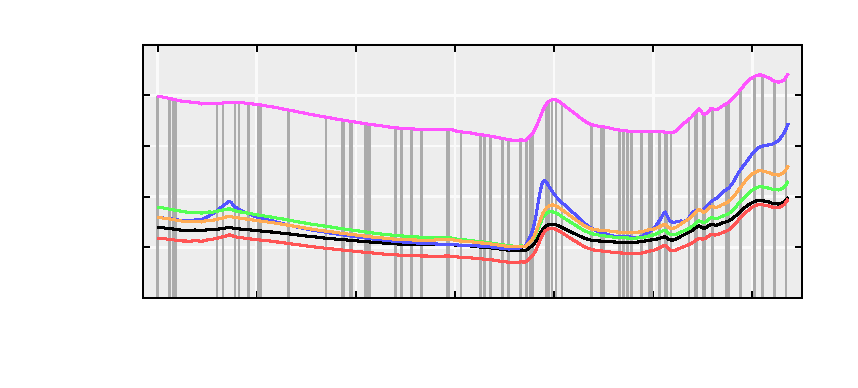
\includegraphics{gp/ms-sa-n-spec-rnd}}%
    \gplfronttext
  \end{picture}%
\endgroup

			\caption{$p^{(\m{N})}$ with $\m{p}^{(\m{N})} = 69$}
			\label{sfig:calib-n}
		\end{subfigure}

		\begin{subfigure}[b]{\textwidth}
			\centering
			% GNUPLOT: LaTeX picture with Postscript
\begingroup
  \makeatletter
  \providecommand\color[2][]{%
    \GenericError{(gnuplot) \space\space\space\@spaces}{%
      Package color not loaded in conjunction with
      terminal option `colourtext'%
    }{See the gnuplot documentation for explanation.%
    }{Either use 'blacktext' in gnuplot or load the package
      color.sty in LaTeX.}%
    \renewcommand\color[2][]{}%
  }%
  \providecommand\includegraphics[2][]{%
    \GenericError{(gnuplot) \space\space\space\@spaces}{%
      Package graphicx or graphics not loaded%
    }{See the gnuplot documentation for explanation.%
    }{The gnuplot epslatex terminal needs graphicx.sty or graphics.sty.}%
    \renewcommand\includegraphics[2][]{}%
  }%
  \providecommand\rotatebox[2]{#2}%
  \@ifundefined{ifGPcolor}{%
    \newif\ifGPcolor
    \GPcolorfalse
  }{}%
  \@ifundefined{ifGPblacktext}{%
    \newif\ifGPblacktext
    \GPblacktexttrue
  }{}%
  % define a \g@addto@macro without @ in the name:
  \let\gplgaddtomacro\g@addto@macro
  % define empty templates for all commands taking text:
  \gdef\gplbacktext{}%
  \gdef\gplfronttext{}%
  \makeatother
  \ifGPblacktext
    % no textcolor at all
    \def\colorrgb#1{}%
    \def\colorgray#1{}%
  \else
    % gray or color?
    \ifGPcolor
      \def\colorrgb#1{\color[rgb]{#1}}%
      \def\colorgray#1{\color[gray]{#1}}%
      \expandafter\def\csname LTw\endcsname{\color{white}}%
      \expandafter\def\csname LTb\endcsname{\color{black}}%
      \expandafter\def\csname LTa\endcsname{\color{black}}%
      \expandafter\def\csname LT0\endcsname{\color[rgb]{1,0,0}}%
      \expandafter\def\csname LT1\endcsname{\color[rgb]{0,1,0}}%
      \expandafter\def\csname LT2\endcsname{\color[rgb]{0,0,1}}%
      \expandafter\def\csname LT3\endcsname{\color[rgb]{1,0,1}}%
      \expandafter\def\csname LT4\endcsname{\color[rgb]{0,1,1}}%
      \expandafter\def\csname LT5\endcsname{\color[rgb]{1,1,0}}%
      \expandafter\def\csname LT6\endcsname{\color[rgb]{0,0,0}}%
      \expandafter\def\csname LT7\endcsname{\color[rgb]{1,0.3,0}}%
      \expandafter\def\csname LT8\endcsname{\color[rgb]{0.5,0.5,0.5}}%
    \else
      % gray
      \def\colorrgb#1{\color{black}}%
      \def\colorgray#1{\color[gray]{#1}}%
      \expandafter\def\csname LTw\endcsname{\color{white}}%
      \expandafter\def\csname LTb\endcsname{\color{black}}%
      \expandafter\def\csname LTa\endcsname{\color{black}}%
      \expandafter\def\csname LT0\endcsname{\color{black}}%
      \expandafter\def\csname LT1\endcsname{\color{black}}%
      \expandafter\def\csname LT2\endcsname{\color{black}}%
      \expandafter\def\csname LT3\endcsname{\color{black}}%
      \expandafter\def\csname LT4\endcsname{\color{black}}%
      \expandafter\def\csname LT5\endcsname{\color{black}}%
      \expandafter\def\csname LT6\endcsname{\color{black}}%
      \expandafter\def\csname LT7\endcsname{\color{black}}%
      \expandafter\def\csname LT8\endcsname{\color{black}}%
    \fi
  \fi
  \setlength{\unitlength}{0.0500bp}%
  \begin{picture}(7936.00,3400.00)%
    \gplgaddtomacro\gplbacktext{%
      \csname LTb\endcsname%
      \put(1078,704){\makebox(0,0)[r]{\strut{} 0.3}}%
      \csname LTb\endcsname%
      \put(1078,1190){\makebox(0,0)[r]{\strut{} 0.35}}%
      \csname LTb\endcsname%
      \put(1078,1676){\makebox(0,0)[r]{\strut{} 0.4}}%
      \csname LTb\endcsname%
      \put(1078,2163){\makebox(0,0)[r]{\strut{} 0.45}}%
      \csname LTb\endcsname%
      \put(1078,2649){\makebox(0,0)[r]{\strut{} 0.5}}%
      \csname LTb\endcsname%
      \put(1078,3135){\makebox(0,0)[r]{\strut{} 0.55}}%
      \csname LTb\endcsname%
      \put(1353,484){\makebox(0,0){\strut{} 1400}}%
      \csname LTb\endcsname%
      \put(2304,484){\makebox(0,0){\strut{} 1600}}%
      \csname LTb\endcsname%
      \put(3256,484){\makebox(0,0){\strut{} 1800}}%
      \csname LTb\endcsname%
      \put(4208,484){\makebox(0,0){\strut{} 2000}}%
      \csname LTb\endcsname%
      \put(5160,484){\makebox(0,0){\strut{} 2200}}%
      \csname LTb\endcsname%
      \put(6111,484){\makebox(0,0){\strut{} 2400}}%
      \csname LTb\endcsname%
      \put(7063,484){\makebox(0,0){\strut{} 2600}}%
      \put(176,1919){\rotatebox{-270}{\makebox(0,0){\strut{}$-\lg \varrho(\lambda)$}}}%
      \put(4374,154){\makebox(0,0){\strut{}$\lambda \ [\m{nm}]$}}%
    }%
    \gplgaddtomacro\gplfronttext{%
      \csname LTb\endcsname%
      \put(6587,2892){\makebox(0,0)[r]{\strut{}$\overline{\m{pH}}$}}%
    }%
    \gplbacktext
    \put(0,0){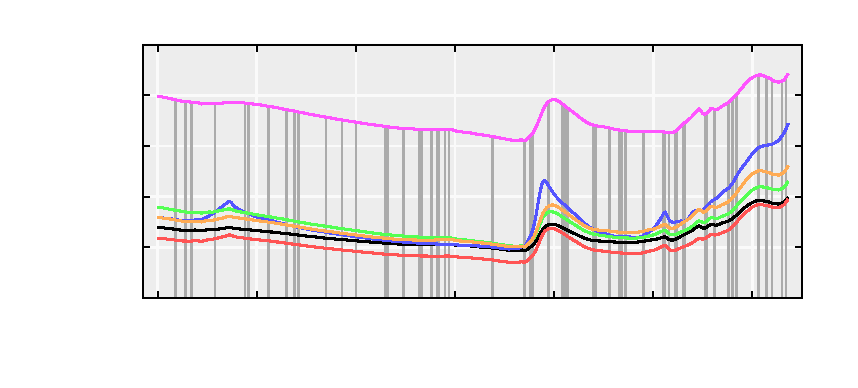
\includegraphics{gp/ms-sa-ph-spec-rnd}}%
    \gplfronttext
  \end{picture}%
\endgroup

			\caption{$\m{pH}$ with $\m{p}^{(\m{pH})} = 58$}
			\label{sfig:calib-ph}
		\end{subfigure}
		\caption{Displaying the spectra from figure \ref{fig:soil-spec-rnd} with wavelength included in the selected models for each response highlighted by vertical grey lines}
	\end{figure}

% section

	\section{R Source Code}
\label{sec:r-source-code}

\lstinputlisting[basicstyle=\footnotesize\ttfamily, frame=single]{code/modelselect.R}
\clearpage
\lstinputlisting[basicstyle=\footnotesize\ttfamily, frame=single]{code/simulation.R}
\clearpage
\lstinputlisting[basicstyle=\footnotesize\ttfamily, frame=single]{code/helper.R}
\lstinputlisting[basicstyle=\footnotesize\ttfamily, frame=single]{code/spse.R}
\clearpage
\lstinputlisting[basicstyle=\footnotesize\ttfamily, frame=single]{code/main.R}


% section r-source-code
	
	\newpage
\thispagestyle{empty}
\section*{Eigenständigkeitserklärung}
\bigskip


Hiermit bestätigen wir, dass wir die vorliegende Arbeit selbständig verfasst und keine anderen als die angegebenen Hilfsmittel verwendet haben. Die Stellen der Arbeit, die dem Wortlaut oder dem Sinn nach anderen Werken (dazu zählen auch Internetquellen) entnommen sind, wurden unter Angabe der Quelle kenntlich gemacht.

\vspace{1 cm}

\noindent
Jena, 01. April 2019

\vspace{1 cm}
Ferdinand Rewicki \hspace{3 cm} Moritz Preuß \hspace{3 cm} Tobias Giesemann


\end{document}
